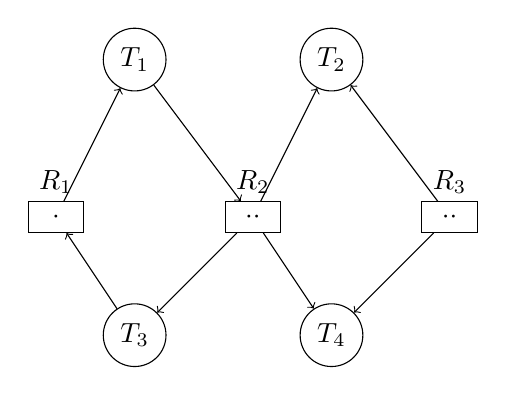
\begin{tikzpicture}
\tikzstyle{label} = [above,yshift=5pt];
\tikzstyle{res}=[minimum width=20pt,minimum height=5pt,draw];
\tikzstyle{pro}=[circle,draw];
\tikzstyle{alloc}=[->];
\node [res] (v1) at (-3,1) {$\cdot$};
\node [label] at (v1) {$R_1$};
\node [pro] (v2) at (-2,3) {$T_1$};

\node [pro] (v4) at (0.5,3) {$T_2$};
\node [pro] (v5) at (-2,-0.5) {$T_3$};
\node [res] (v3) at (-0.5,1) {$\cdot\cdot$};
\node [label] at (v3) {$R_2$};
\node [pro] (v6) at (0.5,-0.5) {$T_4$};
\draw [alloc] (v1) edge (v2);

\node (v7) [res] at (2,1) {$\cdot\cdot$};
\node [label] at (v7) {$R_3$};

\draw [alloc] (v2) edge (v3);
\draw [alloc] (v3) edge (v4);
\draw [alloc] (v7) edge (v4);
\draw [alloc] (v3) edge (v5);
\draw [alloc] (v5) edge (v1);
\draw [alloc] (v3) edge (v6);
\draw [alloc] (v7) edge (v6);
\end{tikzpicture}
